%%%%%%%%%%%%%%%%%%%%% chapter.tex %%%%%%%%%%%%%%%%%%%%%%%%%%%%%%%%%
%
% sample chapter
%
% Use this file as a template for your own input.
%
%%%%%%%%%%%%%%%%%%%%%%%% Springer-Verlag %%%%%%%%%%%%%%%%%%%%%%%%%%
%\motto{Use the template \emph{chapter.tex} to style the various elements of your chapter content.}

\chapter{Rosetta Code Tasks starting with O}

\section*{Object serialization}


Create a set of data types based upon
\emph{inheritance}. Each data type or class should
have a print command that displays the contents of an instance of that
class to standard output. Create instances of each class in your
inheritance hierarchy and display them to standard output. Write each of
the objects to a file named \emph{objects.dat} in binary form using
serialization or marshalling. Read the file \emph{objects.dat} and print
the contents of each serialized object.

\begin{wideverbatim}

The built-in function [http://software-lab.de/doc/refP.html#pr pr] serializes
any kind of data, and [http://software-lab.de/doc/refR.html#rd rd] reads it
back. This functionality is also used internally for database access and
interprocess-communication.

(class +Point)
# x y

(dm T (X Y)
   (=: x (or X 0))
   (=: y (or Y 0)) )

(dm print> ()
   (prinl "Point " (: x) "," (: y)) )

(class +Circle +Point)
# r

(dm T (X Y R)
   (super X Y)
   (=: r (or R 0)) )

(dm print> ()
   (prinl "Circle " (: x) "," (: y) "," (: r)) )

(setq
   P (new '(+Point) 3 4)
   C (new '(+Circle) 10 10 5) )

(print> P)
(print> C)

(out "objects.dat"
   (pr (val P) (getl P))
   (pr (val C) (getl C)) )

(in "objects.dat"
   (putl (setq A (box (rd))) (rd))
   (putl (setq B (box (rd))) (rd)) )

(print> A)
(print> B)

Output:

Point 3,4
Circle 10,10,5
Point 3,4
Circle 10,10,5

\end{wideverbatim}

\pagebreak{}
\section*{Odd word problem}

Write a program that solves the
\href{http://c2.com/cgi/wiki?OddWordProblem}{odd word problem} with the
restrictions given below.

\textbf{Description}: You are promised an input stream consisting of
English letters and punctuations. It is guaranteed that

\begin{itemize}
\item
  the words (sequence of consecutive letters) are delimited by one and
  only one punctuation; that
\item
  the stream will begin with a word; that
\item
  the words will be at least one letter long; and that
\item
  a full stop (.) appears after, and only after, the last word.
\end{itemize}

For example, \texttt{what,is,the;meaning,of:life.} is such a stream with
six words. Your task is to reverse the letters in every other word while
leaving punctuations intact, producing e.g.
``what,si,the;gninaem,of:efil.'', while observing the following
restrictions:

\begin{enumerate}
\item
  Only I/O allowed is reading or writing one character at a time, which
  means: no reading in a string, no peeking ahead, no pushing characters
  back into the stream, and no storing characters in a global variable
  for later use;
\item
  You \textbf{are not} to explicitly save characters in a collection
  data structure, such as arrays, strings, hash tables, etc, for later
  reversal;
\item
  You \textbf{are} allowed to use recursions, closures, continuations,
  threads, coroutines, etc., even if their use implies the storage of
  multiple characters.
\end{enumerate}

\textbf{Test case}: work on both the ``life'' example given above, and
the text \\ \texttt{we,are;not,in,kansas;any,more.}


\begin{wideverbatim}

(de oddWords ()
   (use C
      (loop
         (until (sub? (prin (setq C (char))) "!,.:;?"))
         (T (= "." C))
         (setq C (char))
         (T
            (= "."
               (prin
                  (recur (C)
                     (if (sub? C "!,.:;?")
                        C
                        (prog1 (recurse (char)) (prin C)) ) ) ) ) ) )
   (prinl) ) )

Test:

(in "txt1" (oddWords))
(in "txt2" (oddWords))

Output:

what,si,the;gninaem,of:efil.
we,era;not,ni,kansas;yna,more.

\end{wideverbatim}

\pagebreak{}
\section*{Old lady swalllowed a fly}

Present a program which emits the lyrics to the song
\emph{\href{http://en.wikipedia.org/wiki/There\_Was\_an\_Old\_Lady\_Who\_Swallowed\_a\_Fly}{I
    Knew an Old Lady Who Swallowed a Fly}}, taking advantage of the
repetitive structure of the song's lyrics. This song has multiple
versions with slightly different lyrics, so all these programs might
not emit identical output.

See also: \emph{99 Bottles of Beer}

\begin{wideverbatim}



(de *Dict
   `(chop
      "_ha _c _e _p,/Quite absurd_f_p;_`cat,/Fancy that_fcat;_j`dog,\
         /What a hog_fdog;_l`pig,/Her mouth_qso big_fpig;_d_r,/She just \
         opened her throat_f_r;_icow,/_mhow she_ga cow;_k_o,/It_qrather \
         wonky_f_o;_a_o_bcow,_khorse.../She's dead, of course!/" )
   `(chop "_a_p_b_e ")
   `(chop "/S_t ")
   `(chop " to catch the ")
   `(chop "fly,/But _mwhy s_t fly,/Perhaps she'll die!//_ha")
   `(chop "_apig_bdog,_l`")
   `(chop "spider,/That wr_nj_ntickled inside her;_aspider_b_c")
   `(chop ", to_s a ")
   `(chop "_sed ")
   `(chop "There_qan old lady who_g")
   `(chop "_a_r_bpig,_d")
   `(chop "_acat_b_p,_")
   `(chop "_acow_b_r,_i")
   `(chop "_adog_bcat,_j")
   `(chop "I don't know ")
   `(chop "iggled and ")
   `(chop "donkey")
   `(chop "bird")
   `(chop " was ")
   `(chop "goat")
   `(chop " swallow")
   `(chop "he_gthe") )

(de oldLady (Lst Flg)
   (loop
      (let C (pop 'Lst)
         (cond
            (Flg
               (setq Flg
                  (oldLady (get *Dict (- (char C) 94))) ) )
            ((= "_" C) (on Flg))
            ((= "/" C) (prinl))
            (T (prin C)) ) )
      (NIL Lst) )
   Flg )

(oldLady (car *Dict))

\end{wideverbatim}

\pagebreak{}
\section*{One of n lines in a file}

A method of choosing a line randomly from a file:

\begin{itemize}
\item
  Without reading the file more than once
\item
  When substantial parts of the file cannot be held in memory
\item
  Without knowing how many lines are in the file
\end{itemize}

Is to:

\begin{itemize}
\item
  keep the first line of the file as a possible choice, then
\item
  Read the second line of the file if possible and make it the possible
  choice if a uniform random value between zero and one is less than
  1/2.
\item
  Read the third line of the file if possible and make it the possible
  choice if a uniform random value between zero and one is less than
  1/3.
\end{itemize}

\ldots{}

\begin{itemize}
\item
  Read the Nth line of the file if possible and make it the possible
  choice if a uniform random value between zero and one is less than 1/N
\end{itemize}

\begin{itemize}
\item
  Return the computed possible choice when no further lines exist in the
  file.
\end{itemize}

\begin{description}
\item[Task]
\end{description}

\begin{enumerate}
\item
  Create a function/method/routine called \texttt{one\_of\_n} that given
  \texttt{n}, the number of actual lines in a file, follows the
  algorithm above to return an integer - the line number of the line
  chosen from the file. \\The number returned can vary, randomly, in
  each run.
\item
  Use \texttt{one\_of\_n} in a \emph{simulation} to find what woud be
  the chosen line of a 10 line file simulated 1,000,000 times.
\item
  Print and show how many times each of the 10 lines is chosen as a
  rough measure of how well the algorithm works.
\end{enumerate}

Note: You may choose a smaller number of repetitions if necessary, but
mention this up-front.


\begin{wideverbatim}

(de one-of-n (N)
   (let R 1
      (for I N
         (when (= 1 (rand 1 I))
            (setq R I) ) )
      R ) )

(let L (need 10 0)
   (do 1000000
      (inc (nth L (one-of-n 10))) )
   L )

Output:

-> (99893 100145 99532 100400 100263 100229 99732 100116 99709 99981)

\end{wideverbatim}

\pagebreak{}
\section*{One-dimensional cellular automata}

Assume an array of cells with an initial distribution of live and dead
cells, and imaginary cells off the end of the array having fixed values.

Cells in the next generation of the array are calculated based on the
value of the cell and its left and right nearest neighbours in the
current generation. If, in the following table, a live cell is
represented by 1 and a dead cell by 0 then to generate the value of the
cell at a particular index in the array of cellular values you use the
following table:

\begin{verbatim}
000 -> 0  # 
001 -> 0  #
010 -> 0  # Dies without enough neighbours
011 -> 1  # Needs one neighbour to survive
100 -> 0  #
101 -> 1  # Two neighbours giving birth
110 -> 1  # Needs one neighbour to survive
111 -> 0  # Starved to death.
\end{verbatim}



\begin{wideverbatim}

(let Cells (chop "_###_##_#_#_#_#__#__")
   (do 10
      (prinl Cells)
      (setq Cells
         (make
            (link "_")
            (map
               '((L)
                  (case (head 3 L)
                     (`(mapcar chop '("___" "__#" "_#_" "#__" "###"))
                         (link "_") )
                     (`(mapcar chop '("_##" "#_#" "##_"))
                        (link "#") ) ) )
               Cells )
            (link "_") ) ) ) )

Output:

_###_##_#_#_#_#__#__
_#_#####_#_#_#______
__##___##_#_#_______
__##___###_#________
__##___#_##_________
__##____###_________
__##____#_#_________
__##_____#__________
__##________________
__##________________

\end{wideverbatim}

\pagebreak{}
\section*{OpenGL}

In this task, the goal is to display a smooth shaded triangle with
OpenGL.

\begin{figure}[H]
\centering
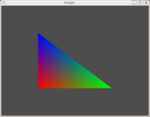
\includegraphics[scale=.6]{graphics/150px-Triangle.png}
\end{figure}

% \emph{\includegraphics[scale=.6]{graphics/magnify-clip.png}}

Triangle created using C example compiled with \emph{GCC} 4.1.2 and
\emph{freeglut3}.


\begin{wideverbatim}

This is for the 64-bit version.

(load "@lib/openGl.l")

(glutInit)
(glutInitWindowSize 400 300)
(glutCreateWindow "Triangle")

(displayPrg
   (glClearColor 0.3 0.3 0.3 0.0)
   (glClear (| GL_COLOR_BUFFER_BIT GL_DEPTH_BUFFER_BIT))
   (glShadeModel GL_SMOOTH)
   (glLoadIdentity)
   (glTranslatef -15.0 -15.0 0.0)
   (glBegin GL_TRIANGLES)
   (glColor3f 1.0 0.0 0.0)
   (glVertex2f 0.0 0.0)
   (glColor3f 0.0 1.0 0.0)
   (glVertex2f 30.0 0.0)
   (glColor3f 0.0 0.0 1.0)
   (glVertex2f 0.0 30.0)
   (glEnd)
   (glFlush) )

(reshapeFunc
   '((Width Height)
      (glViewport 0 0 Width Height)
      (glMatrixMode GL_PROJECTION)
      (glLoadIdentity)
      (glOrtho -30.0 30.0 -30.0 30.0 -30.0 30.0)
      (glMatrixMode GL_MODELVIEW) ) )

# Exit upon mouse click
(mouseFunc '((Btn State X Y) (bye)))

(glutMainLoop)

\end{wideverbatim}

\pagebreak{}
\section*{Optional parameters}

Define a function/method/subroutine which sorts a sequence (``table'')
of sequences (``rows'') of strings (``cells''), by one of the strings.
Besides the input to be sorted, it shall have the following optional
parameters:

\begin{center}\rule{3in}{0.4pt}\end{center}

\begin{itemize}
\item \textbf{ordering} A function specifying the ordering of strings;
  lexicographic by default.
\item \textbf{column} An integer specifying which string of each row
  to compare; the first by default.
\item \textbf{reverse} Reverses the ordering.
\end{itemize}

\begin{center}\rule{3in}{0.4pt}\end{center}

This task should be considered to include both positional and named
optional parameters, as well as overloading on argument count as in Java
or selector name as in Smalltalk, or, in the extreme, using different
function names. Provide these variations of sorting \textbf{in whatever
way is most natural to your language}. If the language supports both
methods naturally, you are encouraged to describe both.

Do not implement a sorting algorithm; this task is about the interface.
If you can't use a built-in sort routine, just omit the implementation
(with a comment).

See also:

\begin{itemize}
\item
  \emph{Named Arguments}
\end{itemize}



\begin{wideverbatim}

(de sortTable (Tbl . @)
   (let (Ordering prog  Column 1  Reverse NIL)  # Set defaults
      (bind (rest)                              # Bind optional params
         (setq Tbl
            (by '((L) (Ordering (get L Column)))
               sort
               Tbl ) )
         (if Reverse (flip Tbl) Tbl) ) ) )

Output:

(de *Data ("a" "bcdef" "X") (" " "qrst" "z") ("zap" "zip" "Zot"))

: (sortTable *Data)
-> ((" " "qrst" "z") ("a" "bcdef" "X") ("zap" "zip" "Zot"))

: (sortTable *Data '(Reverse . T))
-> (("zap" "zip" "Zot") ("a" "bcdef" "X") (" " "qrst" "z"))

: (sortTable *Data '(Column . 2) '(Ordering . length))
-> (("zap" "zip" "Zot") (" " "qrst" "z") ("a" "bcdef" "X"))

: (sortTable *Data '(Ordering . uppc) '(Column . 3))
-> (("a" "bcdef" "X") (" " "qrst" "z") ("zap" "zip" "Zot"))

\end{wideverbatim}

\pagebreak{}
\section*{Order two numerical lists}

Write a function that orders two lists or arrays filled with numbers.
The function should accept two lists as arguments and return
\texttt{true} if the first list should be ordered before the second,
and \texttt{false} otherwise.

The order is determined by
\href{http://en.wikipedia.org/wiki/Lexicographical\_order\#Ordering\_of\_sequences\_of\_various\_lengths}{lexicographic
order}: Comparing the first element of each list. If the first elements
are equal, then the second elements should be compared, and so on, until
one of the list has no more elements. If the first list runs out of
elements the result is \texttt{true}. if the second list or both run out
of elements the result is \texttt{false}.


\begin{wideverbatim}

The built-in comparison functions already do this (not only for lists of
numbers, but for any arbitrary data type).

: (> (1 2 0 4 4 0 0 0) (1 2 1 3 2))
-> NIL

\end{wideverbatim}

\pagebreak{}
\section*{Ordered Partitions}


In this task we want to find the ordered partitions into fixed-size
blocks. This task is related to \emph{Combinations}
in that it has to do with discrete mathematics and moreover a helper
function to compute combinations is (probably) needed to solve this
task.

\emph{p}\emph{a}\emph{r}\emph{t}\emph{i}\emph{t}\emph{i}\emph{o}\emph{n}\emph{s}(\emph{a}\emph{r}\emph{g}\textsubscript{1},\emph{a}\emph{r}\emph{g}\textsubscript{2},\ldots{},\emph{a}\emph{r}\emph{g}\textsubscript{\emph{n}})
should generate all distributions of the elements in
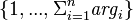
\includegraphics[scale=.6]{graphics/bc37f835564eb6edd3510913644f4582.png}
into \emph{n} blocks of respective size
\emph{a}\emph{r}\emph{g}\textsubscript{1},\emph{a}\emph{r}\emph{g}\textsubscript{2},\ldots{},\emph{a}\emph{r}\emph{g}\textsubscript{\emph{n}}.

Example 1:
\emph{p}\emph{a}\emph{r}\emph{t}\emph{i}\emph{t}\emph{i}\emph{o}\emph{n}\emph{s}(2,0,2)
would create:

\begin{verbatim}
{({1, 2}, {}, {3, 4}), 
 ({1, 3}, {}, {2, 4}), 
 ({1, 4}, {}, {2, 3}), 
 ({2, 3}, {}, {1, 4}), 
 ({2, 4}, {}, {1, 3}), 
 ({3, 4}, {}, {1, 2})}
\end{verbatim}

Example 2:
\emph{p}\emph{a}\emph{r}\emph{t}\emph{i}\emph{t}\emph{i}\emph{o}\emph{n}\emph{s}(1,1,1)
would create:

\begin{verbatim}
{({1}, {2}, {3}), 
 ({1}, {3}, {2}), 
 ({2}, {1}, {3}), 
 ({2}, {3}, {1}), 
 ({3}, {1}, {2}), 
 ({3}, {2}, {1})}
\end{verbatim}

Note that the number of elements in the list is

\begin{figure}[H]
\centering
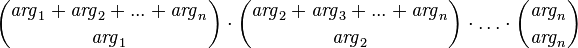
\includegraphics[scale=.6]{graphics/05e249cad1085102aca0ad06c5eb4236.png}
% \caption{\{\textbackslash{}mathit\{arg\}\_1+\textbackslash{}mathit\{arg\}\_2+...+\textbackslash{}mathit\{arg\}\_n
% \textbackslash{}choose \textbackslash{}mathit\{arg\}\_1\}
% \textbackslash{}cdot
% \{\textbackslash{}mathit\{arg\}\_2+\textbackslash{}mathit\{arg\}\_3+...+\textbackslash{}mathit\{arg\}\_n
% \textbackslash{}choose \textbackslash{}mathit\{arg\}\_2\}
% \textbackslash{}cdot \textbackslash{}ldots \textbackslash{}cdot
% \{\textbackslash{}mathit\{arg\}\_n \textbackslash{}choose
% \textbackslash{}mathit\{arg\}\_n\}}
\end{figure}

(see \href{http://en.wikipedia.org/wiki/Binomial\_coefficient}{the
definition of the binomial coefficient} if you are not familiar with
this notation) and the number of elements remains the same regardless of
how the argument is permuted (i.e. the
\href{http://en.wikipedia.org/wiki/Multinomial\_coefficient}{multinomial
coefficient}). Also,
\emph{p}\emph{a}\emph{r}\emph{t}\emph{i}\emph{t}\emph{i}\emph{o}\emph{n}\emph{s}(1,1,1)
creates the permutations of \{1,2,3\} and thus there would be 3! = 6
elements in the list.

Note: Do not use functions that are not in the standard library of the
programming language you use. Your file should be written so that it can
be executed on the command line and by default outputs the result of
\emph{p}\emph{a}\emph{r}\emph{t}\emph{i}\emph{t}\emph{i}\emph{o}\emph{n}\emph{s}(2,0,2).
If the programming language does not support polyvariadic functions pass
a list as an argument.

\pagebreak{}

\textbf{Notation}

Remarks on the used notation for the task in order to understand it
easierly.

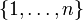
\includegraphics[scale=.6]{graphics/02617b75af4d512caf92071211ac3d6a.png}
denotes the set of consecutive numbers from 1 to \emph{n}, e.g.
\{1,2,3\} if \emph{n} = 3. Σ is the mathematical notation for summation,
e.g.
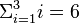
\includegraphics[scale=.6]{graphics/65027d595737121ba207f647f86dfe09.png}
(see also
\href{http://en.wikipedia.org/wiki/Summation\#Capital-sigma\_notation}{{[}1{]}}).
\emph{a}\emph{r}\emph{g}\textsubscript{1},\emph{a}\emph{r}\emph{g}\textsubscript{2},\ldots{},\emph{a}\emph{r}\emph{g}\textsubscript{\emph{n}}
are the arguments --- natural numbers --- that the sought function
receives.

\begin{wideverbatim}

Uses the 'comb' function from [[Combinations#PicoLisp]]

(de partitions (Args)
   (let Lst (range 1 (apply + Args))
      (recur (Args Lst)
         (ifn Args
            '(NIL)
            (mapcan
               '((L)
                  (mapcar
                     '((R) (cons L R))
                     (recurse (cdr Args) (diff Lst L)) ) )
               (comb (car Args) Lst) ) ) ) ) )

Output:

: (more (partitions (2 0 2)))
((1 2) NIL (3 4))
((1 3) NIL (2 4))
((1 4) NIL (2 3))
((2 3) NIL (1 4))
((2 4) NIL (1 3))
((3 4) NIL (1 2))
-> NIL

: (more (partitions (1 1 1)))
((1) (2) (3))
((1) (3) (2))
((2) (1) (3))
((2) (3) (1))
((3) (1) (2))
((3) (2) (1))
-> NIL

\end{wideverbatim}

\pagebreak{}
\section*{Ordered words}

Define an ordered word as a word in which the letters of the word appear
in alphabetic order. Examples include `abbey' and `dirt'.

The task is to find \emph{and display} all the ordered words in this
\href{http://www.puzzlers.org/pub/wordlists/unixdict.txt}{dictionary}
that have the longest word length. (Examples that access the dictionary
file locally assume that you have downloaded this file yourself.) The
display needs to be shown on this page.


\begin{wideverbatim}

(in "unixdict.txt"
   (mapc prinl
      (maxi '((L) (length (car L)))
         (by length group
            (filter '((S) (apply <= S))
               (make (while (line) (link @))) ) ) ) ) )

Output:

abbott
accent
accept
access
accost
almost
bellow
billow
biopsy
chilly
choosy
choppy
effort
floppy
glossy
knotty

\end{wideverbatim}



% %%%%%%%%%%%%%%%%%%%%%%%% referenc.tex %%%%%%%%%%%%%%%%%%%%%%%%%%%%%%
% sample references
% %
% Use this file as a template for your own input.
%
%%%%%%%%%%%%%%%%%%%%%%%% Springer-Verlag %%%%%%%%%%%%%%%%%%%%%%%%%%
%
% BibTeX users please use
% \bibliographystyle{}
% \bibliography{}
%
\biblstarthook{In view of the parallel print and (chapter-wise) online publication of your book at \url{www.springerlink.com} it has been decided that -- as a genreral rule --  references should be sorted chapter-wise and placed at the end of the individual chapters. However, upon agreement with your contact at Springer you may list your references in a single seperate chapter at the end of your book. Deactivate the class option \texttt{sectrefs} and the \texttt{thebibliography} environment will be put out as a chapter of its own.\\\indent
References may be \textit{cited} in the text either by number (preferred) or by author/year.\footnote{Make sure that all references from the list are cited in the text. Those not cited should be moved to a separate \textit{Further Reading} section or chapter.} The reference list should ideally be \textit{sorted} in alphabetical order -- even if reference numbers are used for the their citation in the text. If there are several works by the same author, the following order should be used: 
\begin{enumerate}
\item all works by the author alone, ordered chronologically by year of publication
\item all works by the author with a coauthor, ordered alphabetically by coauthor
\item all works by the author with several coauthors, ordered chronologically by year of publication.
\end{enumerate}
The \textit{styling} of references\footnote{Always use the standard abbreviation of a journal's name according to the ISSN \textit{List of Title Word Abbreviations}, see \url{http://www.issn.org/en/node/344}} depends on the subject of your book:
\begin{itemize}
\item The \textit{two} recommended styles for references in books on \textit{mathematical, physical, statistical and computer sciences} are depicted in ~\cite{science-contrib, science-online, science-mono, science-journal, science-DOI} and ~\cite{phys-online, phys-mono, phys-journal, phys-DOI, phys-contrib}.
\item Examples of the most commonly used reference style in books on \textit{Psychology, Social Sciences} are~\cite{psysoc-mono, psysoc-online,psysoc-journal, psysoc-contrib, psysoc-DOI}.
\item Examples for references in books on \textit{Humanities, Linguistics, Philosophy} are~\cite{humlinphil-journal, humlinphil-contrib, humlinphil-mono, humlinphil-online, humlinphil-DOI}.
\item Examples of the basic Springer style used in publications on a wide range of subjects such as \textit{Computer Science, Economics, Engineering, Geosciences, Life Sciences, Medicine, Biomedicine} are ~\cite{basic-contrib, basic-online, basic-journal, basic-DOI, basic-mono}. 
\end{itemize}
}

\begin{thebibliography}{99.}%
% and use \bibitem to create references.
%
% Use the following syntax and markup for your references if 
% the subject of your book is from the field 
% "Mathematics, Physics, Statistics, Computer Science"
%
% Contribution 
\bibitem{science-contrib} Broy, M.: Software engineering --- from auxiliary to key technologies. In: Broy, M., Dener, E. (eds.) Software Pioneers, pp. 10-13. Springer, Heidelberg (2002)
%
% Online Document
\bibitem{science-online} Dod, J.: Effective substances. In: The Dictionary of Substances and Their Effects. Royal Society of Chemistry (1999) Available via DIALOG. \\
\url{http://www.rsc.org/dose/title of subordinate document. Cited 15 Jan 1999}
%
% Monograph
\bibitem{science-mono} Geddes, K.O., Czapor, S.R., Labahn, G.: Algorithms for Computer Algebra. Kluwer, Boston (1992) 
%
% Journal article
\bibitem{science-journal} Hamburger, C.: Quasimonotonicity, regularity and duality for nonlinear systems of partial differential equations. Ann. Mat. Pura. Appl. \textbf{169}, 321--354 (1995)
%
% Journal article by DOI
\bibitem{science-DOI} Slifka, M.K., Whitton, J.L.: Clinical implications of dysregulated cytokine production. J. Mol. Med. (2000) doi: 10.1007/s001090000086 
%
\bigskip

% Use the following (APS) syntax and markup for your references if 
% the subject of your book is from the field 
% "Mathematics, Physics, Statistics, Computer Science"
%
% Online Document
\bibitem{phys-online} J. Dod, in \textit{The Dictionary of Substances and Their Effects}, Royal Society of Chemistry. (Available via DIALOG, 1999), 
\url{http://www.rsc.org/dose/title of subordinate document. Cited 15 Jan 1999}
%
% Monograph
\bibitem{phys-mono} H. Ibach, H. L\"uth, \textit{Solid-State Physics}, 2nd edn. (Springer, New York, 1996), pp. 45-56 
%
% Journal article
\bibitem{phys-journal} S. Preuss, A. Demchuk Jr., M. Stuke, Appl. Phys. A \textbf{61}
%
% Journal article by DOI
\bibitem{phys-DOI} M.K. Slifka, J.L. Whitton, J. Mol. Med., doi: 10.1007/s001090000086
%
% Contribution 
\bibitem{phys-contrib} S.E. Smith, in \textit{Neuromuscular Junction}, ed. by E. Zaimis. Handbook of Experimental Pharmacology, vol 42 (Springer, Heidelberg, 1976), p. 593
%
\bigskip
%
% Use the following syntax and markup for your references if 
% the subject of your book is from the field 
% "Psychology, Social Sciences"
%
%
% Monograph
\bibitem{psysoc-mono} Calfee, R.~C., \& Valencia, R.~R. (1991). \textit{APA guide to preparing manuscripts for journal publication.} Washington, DC: American Psychological Association.
%
% Online Document
\bibitem{psysoc-online} Dod, J. (1999). Effective substances. In: The dictionary of substances and their effects. Royal Society of Chemistry. Available via DIALOG. \\
\url{http://www.rsc.org/dose/Effective substances.} Cited 15 Jan 1999.
%
% Journal article
\bibitem{psysoc-journal} Harris, M., Karper, E., Stacks, G., Hoffman, D., DeNiro, R., Cruz, P., et al. (2001). Writing labs and the Hollywood connection. \textit{J Film} Writing, 44(3), 213--245.
%
% Contribution 
\bibitem{psysoc-contrib} O'Neil, J.~M., \& Egan, J. (1992). Men's and women's gender role journeys: Metaphor for healing, transition, and transformation. In B.~R. Wainrig (Ed.), \textit{Gender issues across the life cycle} (pp. 107--123). New York: Springer.
%
% Journal article by DOI
\bibitem{psysoc-DOI}Kreger, M., Brindis, C.D., Manuel, D.M., Sassoubre, L. (2007). Lessons learned in systems change initiatives: benchmarks and indicators. \textit{American Journal of Community Psychology}, doi: 10.1007/s10464-007-9108-14.
%
%
% Use the following syntax and markup for your references if 
% the subject of your book is from the field 
% "Humanities, Linguistics, Philosophy"
%
\bigskip
%
% Journal article
\bibitem{humlinphil-journal} Alber John, Daniel C. O'Connell, and Sabine Kowal. 2002. Personal perspective in TV interviews. \textit{Pragmatics} 12:257--271
%
% Contribution 
\bibitem{humlinphil-contrib} Cameron, Deborah. 1997. Theoretical debates in feminist linguistics: Questions of sex and gender. In \textit{Gender and discourse}, ed. Ruth Wodak, 99--119. London: Sage Publications.
%
% Monograph
\bibitem{humlinphil-mono} Cameron, Deborah. 1985. \textit{Feminism and linguistic theory.} New York: St. Martin's Press.
%
% Online Document
\bibitem{humlinphil-online} Dod, Jake. 1999. Effective substances. In: The dictionary of substances and their effects. Royal Society of Chemistry. Available via DIALOG. \\
http://www.rsc.org/dose/title of subordinate document. Cited 15 Jan 1999
%
% Journal article by DOI
\bibitem{humlinphil-DOI} Suleiman, Camelia, Daniel C. O�Connell, and Sabine Kowal. 2002. `If you and I, if we, in this later day, lose that sacred fire...�': Perspective in political interviews. \textit{Journal of Psycholinguistic Research}. doi: 10.1023/A:1015592129296.
%
%
%
\bigskip
%
%
% Use the following syntax and markup for your references if 
% the subject of your book is from the field 
% "Computer Science, Economics, Engineering, Geosciences, Life Sciences"
%
%
% Contribution 
\bibitem{basic-contrib} Brown B, Aaron M (2001) The politics of nature. In: Smith J (ed) The rise of modern genomics, 3rd edn. Wiley, New York 
%
% Online Document
\bibitem{basic-online} Dod J (1999) Effective Substances. In: The dictionary of substances and their effects. Royal Society of Chemistry. Available via DIALOG. \\
\url{http://www.rsc.org/dose/title of subordinate document. Cited 15 Jan 1999}
%
% Journal article by DOI
\bibitem{basic-DOI} Slifka MK, Whitton JL (2000) Clinical implications of dysregulated cytokine production. J Mol Med, doi: 10.1007/s001090000086
%
% Journal article
\bibitem{basic-journal} Smith J, Jones M Jr, Houghton L et al (1999) Future of health insurance. N Engl J Med 965:325--329
%
% Monograph
\bibitem{basic-mono} South J, Blass B (2001) The future of modern genomics. Blackwell, London 
%
\end{thebibliography}

